\documentclass{article}
\usepackage[dvipsnames]{xcolor} % Required for specifying custom colors
% Packages for custom shapes and boxes
\usepackage{tikz} % Required for drawing custom shapes
\usepackage[framemethod=TikZ]{mdframed} % Required for creating the theorem, definition, exercise and corollary boxes
% \newcounter{theo}[section]\setcounter{theo}{0}
\newcounter{theo}[section]\setcounter{theo}{0}
\renewcommand{\thetheo}{\arabic{section}.\arabic{theo}}

\newenvironment{theo}[2][]{%
    \refstepcounter{theo}

    \ifstrempty{#1}%
    % if condition (without title)
    {\mdfsetup{%
            frametitle={%
                    \tikz[baseline=(current bounding box.east),outer sep=0pt]
                    \node[anchor=east,rectangle,fill=black,text=white]
                    {\strut Theorem~\thetheo};}
        }%
        % else condition (with title)
    }{\mdfsetup{%
            frametitle={%
                    \tikz[baseline=(current bounding box.east),outer sep=0pt]
                    \node[anchor=east,rectangle,fill=black,text=white]
                    {\strut Theorem~\thetheo:~#1};}%
        }%
    }%
    % Both conditions
    \mdfsetup{%
        innertopmargin=6pt,innerbottommargin=12pt,linecolor=black,%
        linewidth=2pt,topline=true,%
        frametitleaboveskip=\dimexpr-\ht\strutbox\relax%
    }

    \begin{mdframed}[]\relax}{%
    \end{mdframed}}
 % This file contains the code for the boxes

% Packages for math symbols and images
\usepackage{amssymb} % Math symbols such as \mathbb
\usepackage{graphicx} % Required for including images

% Package for customizing captions
\usepackage{caption}  % Required for customizing captions

\title{Not so Discrete Math}
\author{Christian Rudder}
\date{August 2024}

\begin{document}

\maketitle

\tableofcontents

% Intentionally left blank
\newpage
\thispagestyle{empty}
\mbox{}
\vfill
\begin{center}
    \textit{This page is left intentionally blank.}
\end{center}
\vfill
\newpage

\section{Sets}
\begin{greenbox}
    \textbf{Opening Questions:} What do we call a collection of things?
    does order or repetition matter? Can we contain collection of other collections? Is an empty collection
    considered a collection? How do we count members of a collection, and how do we define them? Can we
    combine collections, and if so, what are those operations?
\end{greenbox}
\subsection{Introduction to Sets}
\hspace*{1em}
In discrete math we work with some group of `things,' a thing or something
we fancily call an \textbf{object}. A group or categorization of objects is called a set.

\begin{theo}[Set]{thm:set}
    Is a collection of objects.
\end{theo}

\noindent
\textbf{For Example:}
\begin{itemize}
    \item $S$ = The set of all students in a classroom.
    \item $A$ = The set of all vowels in the English alphabet.
    \item $\mathbb{Z}$ = The set of all integers.

\end{itemize}
Objects in a \textbf{set} are called \textbf{elements}.

\begin{theo}[Element]{thm:element}
    An object that is a member of a given set.
\end{theo}

\noindent
To expand on the previous example:
\begin{itemize}
    \item $S = \{s_1, s_2, s_3\}$, where $s_1, s_2, s_3$ are students, elements of the set.
    \item $A = \{a, e, i, o, u\}$, where $a, e, i, o, u$ are elements.
    \item $\mathbb{Z} = \{\ldots, -3, -2, -1, 0, 1, 2, 3, \ldots\}$, elements of integer set.
\end{itemize}
Curly braces denote a set, commas separate elements, and
the `$...$' (ellipse) indicates an indefinite continuation, \underline{used only when the pattern \textbf{is clear.}}\\

\newpage

\noindent
There is also notation to denote members of a set.

\begin{theo}[Membership]{thm:membership}
    If $x$ is an element of set $A$, $x \in A$.
    If $x$ is not an element of set $A$, $x \notin A$.
\end{theo}

\noindent
\textbf{For Example:} Given $A = \{a, e, i, o, u\}$,\\
$a \in A$, ``$a$ is an element of $A$,'' and
$b \notin A$, ``$b$ is not an element of $A$.''\\

\noindent
\textbf{Order nor repetition matter:}
\begin{itemize}
    \item $A = \{1, 2, 3\} = \{3, 2, 1\} = \{1, 2, 3, 3, 3, 3, 3\}$.
    \item $B = \{a, b, c\} = \{a, b, c, a, b, c\}$.
\end{itemize}

\begin{theo}[Properties of a Set]{thm:set_props}
    \begin{itemize}
        \item The order of elements do not matter.
        \item Duplicate elements are not counted.
    \end{itemize}
\end{theo}


A subset is a set contained within another set. If the set $B$ is a subset of set $A$,
then every element in $B$ is also in $A$ as shown in Figure \ref{fig:subset}:


\begin{figure}[ht]
    \centering
    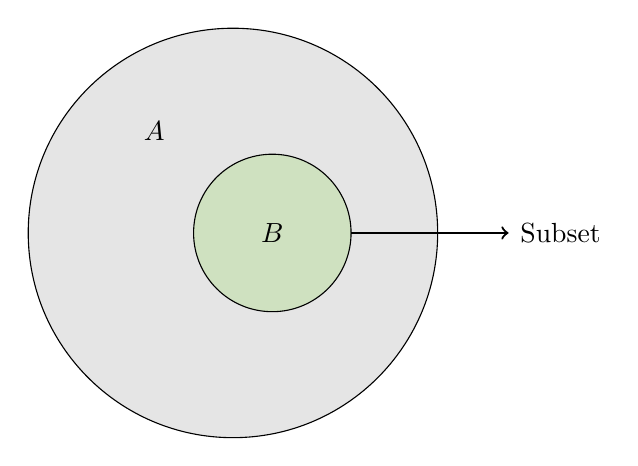
\begin{tikzpicture}
        % Set A
        \draw[fill=gray!20] (0,0) circle (2.6cm);
        \node at (-1,1.3) {$A$};

        % Set B
        \draw[fill=OliveGreen!20] (0.5,0) circle (1cm);
        \node at (0.5,0) {$B$};

        % Subset arrow
        \draw[->, thick] (1.5,0) -- (3.5,0);

        % Subset label
        \node at (4.16,0) {Subset};
    \end{tikzpicture}
    \caption{}
    \label{fig:subset}
\end{figure}


\noindent
Written $B \subseteq A$ or $A \supseteq B$, similar to the less than or
equal to signs `$\leq$' and `$\geq$'.

\newpage

\begin{theo}[Subset]{thm:subset}
    If every element in set $B$ is also in set $A$, then $B$ is a subset of $A$.\\
    Denoted: $B \subseteq A$ or $A \supseteq B$.
\end{theo}

\noindent
\textbf{For Example:}
\begin{itemize}
    \item $\{-1, 0\} \subseteq \{-1, 0, 1, 2, 3\}$
    \item $\{-1, 1, 3\} \subseteq \{-1, 0, 1, 2, 3\}$
    \item $\{-1, 0, 1, 2, 3\} \subseteq \{-1, 0, 1, 2, 3\}$
    \item $\{-1, 7\} \not\subseteq \{-1, 0, 1, 2, 3\}$
\end{itemize}

\underline{$\not\subseteq$ denotes `not a subset of.'}

\vspace{1em}

\noindent
A set with no elements is called the empty set.
\begin{theo}[Empty Set]{thm:empty_set}
    Commonly denoted by $\emptyset$ or $\{\}$, refers to a collection with no objects.
\end{theo}


\noindent
\textbf{Questions:}
\begin{enumerate}
    \item How many elements are in the set  $\{\emptyset\}$?
    \item True or False: $\emptyset \subseteq \{\emptyset\}$.
    \item True or False: $\emptyset \in \{\emptyset\}$.
    \item True or False: $\emptyset \subseteq \emptyset$.
    \item True or False: $\emptyset \subseteq \mathbb{Z}$.
    \item True or False: $\emptyset \in \mathbb{Z}$.
\end{enumerate}
\begin{Tip}
    Mathematicians define things? So can you! Let's define a collection that
    infinitely repeats the string ``bees.'' We will fancily call it\\
    ``\textbf{Bioths Non-determinant Sequence},'' or a $\beta_{seq}$ for short.
    $$\beta_{seq} = \{\textnormal{``bees''}, \textnormal{``bees''}, \textnormal{``bees''}, \textnormal{``bees''},
        \textnormal{``bees''}, \textnormal{``bees''}, \ldots\}$$

    \noindent
    \textbf{Names are names}, no matter how fancy, they were labeled
    by another human, like you. They thought,... ``Damn, this would be a \textit{kick-ass} name.''\\
    Never be intimidated, complex ideas are just groupings of basic concepts.
\end{Tip}
\newpage
\noindent
\textbf{Answers:}
\begin{enumerate}
    \item 1 element, the empty set.
    \item True, the empty set is a subset of $\{\emptyset\}$.
    \item True, the empty set is an element of $\{\emptyset\}$.
    \item True, the empty set is a subset of itself.
    \item True, the empty set is a subset of all sets.
    \item False, the empty set is not an element of the integers.
\end{enumerate}

\vspace{4em}

\noindent
\underline{\textbf{Why (1.):}} \textbf{A collection is an object}. The emptyset is a collection,
a collection without objects. Likewise, a house is still a house without furniture.\\

\noindent
\underline{\textbf{Why (5.):}} Take sets $A=\{\}$ and $B=\{1,2,3\}$\\
By definition of a subset, every element in $A$ must be in $B$. It's difficult to
argue elements in $A$ are indeed in $B$, but it's undeniable that elements in $A$ are not in $B$.
Since our statement cannot be denied, it's \textbf{Vacuously true}.\\

\noindent
\hrulefill\\

\noindent
Say we have an empty box. How many objects do we have? \textbf{Zero}.\\
Put an empty box inside our original box. How many objects now? \textbf{One}!


\begin{figure}[ht]
    $\hspace{.2cm}$
    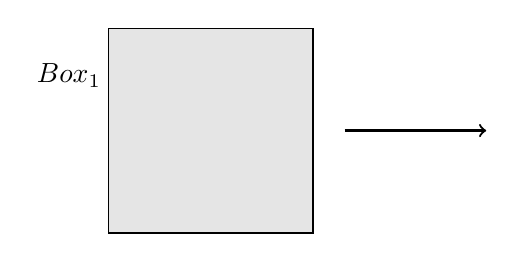
\begin{tikzpicture}
        % Set A
        \draw[fill=gray!20] (0,0) rectangle (2.6cm,2.6cm);
        \node at (-.5,2) {$Box_1$};

        % arrow
        \draw[->, thick] (3,1.3) -- (4.8,1.3);

    \end{tikzpicture}
    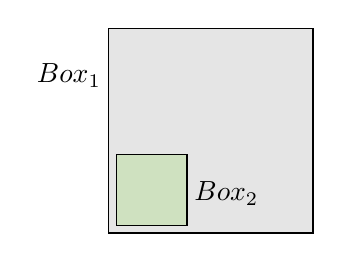
\begin{tikzpicture}
        % Set A
        \draw[fill=gray!20] (0,0) rectangle (2.6cm,2.6cm);
        \node at (-.5,2) {$Box_1$};

        % Set B
        \draw[fill=OliveGreen!20] (1,1) rectangle (.1cm,.1cm);
        \node at (1.5,0.5) {$Box_2$};

        \hfill
    \end{tikzpicture}
    \caption{\centering \underline{$Box_1$ contains 1 object,} which is $Box_2$, an empty box. Hence $\quad$
        $Box_1$ represents $\{\{\}\}$ or $\{\emptyset\}$.}
    \label{fig:empty_box}
\end{figure}

\noindent
\hrulefill\\

\newpage
\noindent
Counting the number of elements in a set is called the \textbf{cardinality} of the set.
\begin{theo}[Cardinality]{thm:cardinality}
    The number of elements in a set.\\
    Denoted over a set $A$ as $|A|$.
\end{theo}

\noindent
\textbf{For Example:}
\begin{itemize}
    \item $A = \{1, 2, 3\}$, $|A| = 3$.
    \item $B = \{a, e, i, o, u\}$, $|B| = 5$.
    \item $\mathbb{Z}$ the set of all integers, $|\mathbb{Z}| = \infty$.
\end{itemize}

\noindent
\textbf{Questions:}\\
What are the cardinalities of the following sets?
\begin{enumerate}
    \item $|\{1,2,3\}|$
    \item $|\emptyset|$
    \item $|\{\}|$
    \item $|\{\emptyset\}|$
    \item $|\{1,\{2,3\}\}|$
    \item $|\{1,2,2,3,3,3\}|$
\end{enumerate}

\vspace{1em}

\noindent
\textbf{Try to think about the answer before looking at the solution.}\\
Things stick when you struggle.\\

\begin{Tip}
    Whenever you approach a problem, always break things down into simple components.
    ``What defines a set? What defines an element? What defines a subset? What defines cardinality?''\\
\end{Tip}

\noindent
\textbf{Answers:}
\begin{enumerate}
    \item 3
    \item 0
    \item 0
    \item 1
    \item 2
    \item 3
\end{enumerate}

\newpage

\noindent
Explicitly defining a set, say $\{1, 2, 3, ...\}$, is called \textbf{set-roster notation}.\\
\textbf{set-builder notation} enables us to create more complex definitions.

\begin{theo}[Set-Builder Notation]{thm:set_builder}
    General form: $\{x \mid P(x)\}$,
    \begin{itemize}
        \item $x$ = defines some variable.
        \item $``\mid"$ = is short hand for ``such that.''
        \item $P(x)$ = describes the properties $x$ must satisfy.
    \end{itemize}
\end{theo}

\noindent
\textbf{For Example:} Lets define the set of even integers\\
\vspace{-1em}
\begin{itemize}
    \item $\{x \mid x \textnormal{ is an even integer}\}$: ``$x$, such that, $x$ is an even integer.''
    \item $\{x \in \mathbb{Z} \mid x \textnormal{ is even}\}$: ``$x$ in Integers, such that, $x$ is an even.''
    \item $\{x \in \mathbb{Z} \mid x \textnormal{ is not odd}\}$: ``$x$ in Integers, such that, $x$ is not odd.''
\end{itemize}

\noindent
\underline{\textbf{It's important to define exactly what variables are.}}
In the above, $x$ was stated directly as an integer. If not, x could be \underline{\textbf{water-balloons} or \textbf{puppies}.}

\subsection{Set Operations}

The combination of $A=\{1,2,3\}$ and $B=\{a,b,c\}$ in order pairs are:
$$(1,a), (1,b), (1,c), $$
$$(2,a), (2,b), (2,c), $$
$$(3,a), (3,b), (3,c)$$

\noindent
Putting the above objects in a set yields the \textbf{Cartesian} product of $A$ and $B$.

% do Union, Intersection, Subraction

\begin{theo}[Cartesian]{thm:cartesian}
    The Cartesian product of two sets $A$ and $B$ is the set of all possible order
    pairs of elements from $A$ and $B$.\\\\
    Denoted: $A \times B$.
\end{theo}

\noindent
\textbf{For Example:}
\begin{itemize}
    \item $\{1, 2\} \times \{a, b\}$, then $A \times B = \{(1,a), (1,b), (2,a), (2,b)\}$.
    \item $A = \{1,2\}, B = \emptyset$, then $A \times B = \emptyset$. $B$ is empty, there is nothing to pair.
    \item $A = \{1\}, B = \{\emptyset\}$, then $A \times B = \{(1,\emptyset)\}$. $B$ contains 1 object to pair.
\end{itemize}
\textbf{Note Figure \ref{fig:empty_box}} from the previous section if the above caused confusion.



\begin{greenbox}
    \textbf{Summary:} A \textbf{set} is a collection of `things' or objects. An object that is a member of a set is an
    \textbf{element} $4\in\mathbb{Z}$. In a set \textbf{order and
        repetition do not matter}. Sets can contain other sets, these subsections/slices/portions are
    called \textbf{subsets}. An \textbf{empty set} is denoted $\emptyset$ or $\{\}$. \textbf{Cardinality} is the element
    count of a set, it does not count sets beyond the top layer. $\{1, {2, 3}\}$ has a cardinality of 2, not 3.
    \textbf{Set-roster} notation is the explicit listing of a set like $\{...,1,2,3,...\}$. \textbf{Set-builder}
    notation is the description of a set $\{x\in \mathbb{Z} | x \textbf{ is even}\}$. Combining two sets is called a \textbf{union},
    the \textbf{intersection} is the common elements between two sets. The \textbf{cartesian product} of two sets is the set of all possible
    ordered pairs. The \textbf{difference} between sets $A$ and $B$ are elements in $A$ that are not in $B$. There
    are many more operations that we could discuss, but we will just stick to these for now.
\end{greenbox}

\begin{graybox}
    \textbf{Comments:} In or out of math, we talk about sets. In conversations,\\
    ``yeah that thing!" ``sorry, what thing?"
    Those people: are we talking about the group or a sub-group of those people. Will we make generalizations?
    Will we be specific? To draw connections, Humans $\in$
    Earth $\in$ Universe. Organizing files, sub-folder to sub-folder. Everything is a set of something.
\end{graybox}
\vspace{1em}

\newpage
\section{Functions}
\subsection{Introduction to Functions}
To talk about functions, is to talk about relationships. Take the `<' sign, this is a relationship.
$x < y$ means $x$ relates to $y$, such that $x$ is less than $y$.\\

\noindent
Let $A=\{1,2,3,4\}$ and $B=\{3,4,5,6\}$\\

\begin{tikzpicture}
    % Draw the sets
    \draw[black] (-3,0) ellipse (1.5 and 2.5);
    \draw[black] (2,0) ellipse (1.5 and 2.5);

    % Labels for the elements in the first set
    \node at (-3,1.5) {1};
    \node at (-3,.5) {2};
    \node at (-3,-.5) {3};
    \node at (-3,-1.5) {4};
    \node at (2,-2.5) {$A$};

    % Labels for the elements in the second set
    \node at (2,1.5) {3};
    \node at (2,.5) {4};
    \node at (2,-.5) {5};
    \node at (2,-1.5) {6};

    % Draw the arrow
    \draw[->, purple] (-1.5,0.5) .. controls (0,1) .. (1.5,0);

\end{tikzpicture}



\vspace{2em}
\begin{greenbox}
    \begin{spacing}{1.5}
        \textbf{Summary: } A \textbf{function} is a \textbf{relationship} between two sets. A set for which we use
        as an input, and a set that will house our outputs. A relationship can be described in
        ordered pairs, take sets $A$ and $B$, over some relation $R$, $x\in A$ relates to $y\in B$
        such that $(x,y)\in R$. The ordered pairs in a \underline{relation is a subset of $A\times B$},
        which includes the emptyset.\\

        \noindent
        A function takes in one input and produces one output. The set of all our inputs is called the
        \textbf{domain}, the set of our outputs the \textbf{codomain}. The set of all possible mappings
        from the domain to the codomain is called the \textbf{range}.\\

        \noindent
        If elements in the codomain all have a mapping, the function is \textbf{onto} or\\
        \textbf{surjective}. If elements in the codomain have a unique mapping, the function is
        \textbf{one-to-one} or \textbf{injective}.
        If a function is both \textbf{onto} and \textbf{one-to-one}, it is \textbf{bijective}.
    \end{spacing}
\end{greenbox}


\newpage

\section{Logic}
\subsection{Introduction to Logic}
\vspace{1em}
Observe the claim below:
\vspace{1em}
\begin{center}
    \Large
    \textit{``You're a rotten cook and your breath is sickly."}
\end{center}
\vspace{1em}

\noindent
This \textbf{assertion} is a \textbf{statement} or \textbf{proposition} that is either \underline{\textbf{TRUE} or \textbf{FALSE}}.\\

\vspace{-1em}
\begin{Note}
    \textbf{Note:} claim, assertion, statement, and proposition are all synonyms.
\end{Note}

\vspace{1em}
\noindent
\textbf{Most Importantly:}
\begin{itemize}
    \item Am I actually a rotten cook?
    \item Is my breath really that sickly?
\end{itemize}

\noindent
We can boil down these two propositions to the following:
\begin{itemize}
    \item $R$: You're a rotten cook
    \item $S$: Your breath is sickly
\end{itemize}

\vspace{1em}
\noindent
The original claim can be rewritten as:
\begin{itemize}
    \item ``$R$ and $S$'' formally written, ``$R \land S$'', ``$\land$'' shorthand for ``AND.''\\
          \underline{\textbf{Both} proposition must be true} for the claim to be true.
\end{itemize}

\vspace{1em}
\noindent
Altering the claim to \textit{``You're a rotten cook or your breath is sickly''} yields:
\begin{itemize}
    \item ``$R$ or $S$'' formally written, ``$R \lor S$'', ``$\lor$'' shorthand for ``OR.''\\
          \underline{\textbf{At least one} of the proposition must me true} for the claim to be true.\\\\
          ``\textit{Maybe you're a rotten cook, maybe your breath is sickly, maybe both}.''
\end{itemize}

\begin{Tip}
    To remember the difference between ``$\land$'' and ``$\lor$'', think: $\land$ looks like an ``A''
    without the line for ``AND''.\\

    \noindent
    Also remember ``And'' is CONJUNCTION, ``OR'' is DISJUNCTION. To
    help, think conjunction means ``conjoin'' to join together,\\ ``I'm putting together
    one and one, I'm \textit{conjoining} them.''\\
\end{Tip}

\noindent
Observe the claim below:
\vspace{1em}
\begin{center}
    \Large
    \textit{``I'm not a rotten cook, but I admit my breath is sickly."}
\end{center}
\vspace{1em}

\noindent
The above states, ``Not $R$'' formally written, ``$\neg R$'', ``$\neg$'' shorthand for ``NOT''.
\underline{``but'' in this context is a conjunction.} The claim writes as: ``$\neg R \land S$''.\\

\begin{Tip}
    Try to uncover what a statement is truly saying, not literally.
    In language we often obfuscate sentences to hide intent or to be more polite.\\
\end{Tip}

\noindent
Observe the claim below:
\vspace{1em}
\begin{center}
    \Large
    \textit{``Either I'm a rotten cook or my breath is sickly,\\ not both."}
\end{center}
\vspace{1em}

\noindent
This is an example of the \textbf{exclusive OR} (XOR), we'll use the symbol ``$\oplus$''.\\
Written as ``$R \oplus S$'', \underline{\textbf{only one} of the proposition can be true, not both.}\\

\noindent
This is more obvious in statements such as:
\begin{itemize}
    \item ``They either went to the party or stayed home.''
    \item ``You are either with me or against me.''
    \item ``They either bought lunch or saved their money.''
\end{itemize}

\noindent
We call ``$\land, \lor, \neg, \oplus$'', \textbf{logical operators}.

\begin{Def}[Logical Operators]{def:logical}
    A symbol that represents a logical operation.
    \begin{itemize}
        \item $\land$: AND, both must be true.
        \item $\lor$: OR, at least one must be true.
        \item $\neg$: NOT, negation, opposite.
        \item $\oplus$: XOR, exclusive OR, either or, but not both.
    \end{itemize}
\end{Def}

\newpage

\noindent
\subsection{Statements vs. Predicates:}
Below reads, \underline{\textbf{``4 is less than 2.''} This is false}, but still \textbf{is a statement}:
\begin{center}
    \large
    $4<2$
\end{center}
A statement evaluates to either true or false, \textbf{predicates don't}. Such as:
\begin{center}
    \large
    $x<2$
\end{center}
\textbf{This is a predicate}, it's neither true or false until we assign a value to $x$.\\

\begin{Def}[Proposition]{def:proposition}
    A statement that is either true or false, independent of any variables.
\end{Def}
\begin{Def}[Predicate]{def:predicate}
    A statement where its truth values depend on one or more variables.
\end{Def}


\subsection{Truth Tables}
Writing whole sentences in logic can be cumbersome even in their reduced logical forms.
So we use \textbf{truth tables} to help keep track our evaluations.\\

\noindent
To demonstrate, let's use a table to show the values $P$ and $\neg P$\\
Our goal is to \underline{find all possible values} of $P$ to then evaluate $\neg P$.\\
Let's take that concept and evaluate $P$ and $Q$ for ``$P \land Q$'' and ``$P \lor Q$.''\\

\begin{center}
    \begin{tabular}{|c|c|}
        \hline
        \rowcolor{OliveGreen!10}
        $P$ & $\neg P$ \\
        \hline
        T   & F        \\
        F   & T        \\
        \hline
    \end{tabular}
\end{center}
\noindent
$T$ = ``True'' and $F$ = ``False'', we refer to these truth values as \underline{\textbf{booleans}}.\\


\begin{Def}[Boolean]{def:boolean}
    A Boolean is a value that can only be either true or false.
\end{Def}

\newpage

\noindent
Our goal here is to find all possible value combinations of $P$ and $Q$ to then evaluate $P \land Q$ and $P \lor Q$.\\


\begin{center}
    \begin{tabular}{|c|c|c|c|}
        \hline
        \rowcolor{OliveGreen!10}
        $P$ & $Q$ & $P \land Q$ & $P \lor Q$ \\
        \hline
        T   & T   & T           & T          \\
        T   & F   & F           & T          \\
        F   & T   & F           & T          \\
        F   & F   & F           & F          \\
        \hline
    \end{tabular}
\end{center}

We will read this table's $P$ then $Q$ boolean values respectively:
\begin{enumerate}
    \item $T$ then $T$, So $T\land T = T$, and $T\lor T = T$.
    \item $T$ then $F$, So $T\land F = F$, and $T\lor F = T$.
    \item $F$ then $T$, So $F\land T = F$, and $F\lor T = T$.
    \item $F$ then $F$, So $F\land F = F$, and $F\lor F = F$.
\end{enumerate}

\begin{Tip}
    When working with new concepts, ask yourself what was going through the creator's mind.
    Try to understand the logic and intuition behind concepts rather than memorizing them.
    So when you forget, you'll be able to derive the concept from scratch, or consider a new novel idea.\\
\end{Tip}

\subsection{Boolean Algebra\\ \& Logical Equivalences}
\vspace{1em}

In digital systems we manipulate binary values to evaluate logic. These systems use
states of \underline{``on'' and ``off'' to represent 1 (true) and 0 (false).}\\

\noindent
This is identical to the propositional logic we've been discussing. Observe:\\
\begin{center}
    \begin{tabular}{c c c}
        Boolean Algebra &     & Propositional Logic \\
        \hline
        $\bar{x}$       & NOT & $\neg x$            \\
        $x \cdot y$     & AND & $x \land y$         \\
        $x + y$         & OR  & $x \lor y$          \\
        $x \oplus y$    & XOR & $x \oplus y$        \\
        \hline
    \end{tabular}
\end{center}

\begin{Note}
    \textbf{Note:} XOR in programming is often represented by the caret symbol `$^\wedge $'.
\end{Note}

\noindent
This is the basis for logic gates and circuits, of which we will not discuss here.\\

\newpage

\noindent
Lets use the following truth table to demonstrate boolean algebra conversion:\\
\begin{center}
    \begin{tabular}{|c|c|c|}
        \hline
        \rowcolor{OliveGreen!10}
        $P$ & $Q$ & $f(x)$ \\
        \hline
        T   & T   & F      \\
        T   & F   & T      \\
        F   & T   & F      \\
        F   & F   & T      \\
        \hline
    \end{tabular}
\end{center}

\begin{tabular}{cc|l}
    \textbf{DNF}                                  & \textbf{CNF}                                 &                     \\
    \hline
    $(P \land \neg Q) \lor (\neg P \land \neg Q)$ & $(\neg P \lor \neg Q) \land (P \lor \neg Q)$ & Propositional Logic \\
    $(P \cdot \bar{Q}) + (\bar{P} \cdot \bar{Q})$ & $(\bar{P} + \bar{Q}) \cdot (P + \bar{Q})$    & Boolean Algebra     \\
    \hline
\end{tabular}

\vspace*{2em}

\noindent
We say \underline{$(P\bar{Q}) + (\bar{P} \bar{Q})$ is \textbf{equivalent} to $(\bar{P} + \bar{Q}) (P + \bar{Q})$.}
This doesn't mean they are syntactically the same or re-arrangeable to match. Rather that they evaluate to the same truth values.\\

\noindent
I.e, we could swap out $f(x)$ for either of the two expressions and \underline{the truth table remains the same.}\\

\begin{Note}
    \textbf{Note:} the dot refers to multiplication so ``$P\cdot Q$'' is ``$PQ$'', they are one and the same.
\end{Note}

\begin{Def}[Logical Equivalence]{def:log_equiv}
    Two expressions are equivalent if they evaluate to the same truth values.\\
    Denoted: $P \equiv Q$.
\end{Def}

\noindent
Obverse the claim:
\begin{center}
    \Large
    \textit{``If you don't study, then you won't pass.''}
\end{center}

This is an example of a \textbf{conditional statement}. Let's break the statement down:
\begin{itemize}
    \item \textbf{S} to study.
    \item \textbf{P} to pass.
\end{itemize}

\noindent
The statement says, ``$\neg S$ \textbf{implies} $\neg P$'', i.e.,
``$\neg S$ \textbf{then} $\neg P$'', formally written as ``$\neg S \rightarrow \neg P$.''\\

\newpage

\noindent
This type of statement is called an \textbf{implication}.
\begin{Def}[Implication]{def:imp}
    A conditionally statement of the form, if $P$ then $Q$.\\
    Denoted: $P \rightarrow Q$.
\end{Def}

\noindent
Observe the following truth table for the implication:

\begin{center}
    \begin{tabular}{|c|c|c|}
        \hline
        \rowcolor{OliveGreen!10}
        $P$ & $Q$ & $P \rightarrow Q$ \\
        \hline
        T   & T   & T                 \\
        T   & F   & F                 \\
        F   & T   & T                 \\
        F   & F   & T                 \\
        \hline
    \end{tabular}
\end{center}

\noindent
Think of the implication as holding a promise:
\begin{itemize}
    \item If the promise to do something, and it gets done, I held my promise (true).
    \item If I promise to do something, and it doesn't get done, I broke my promise (false).
    \item If I never promised to do anything, then I can't break my promise (true).
\end{itemize}
The last statement is true because \underline{there was no promise to break,} hence, it's \textbf{Vacuously True}.\\
Likewise, you cannot deny my claim if I never made one.\\

\begin{Note}
    \textbf{Note:} We saw a \textbf{vacuously true} statement before when saying ``$\emptyset$ is a subset of all sets.''
    As it's impossible to deny that nothing is a part of something.
\end{Note}

\noindent
It actually turns out $P \rightarrow Q$ is equivalent to $\neg P \lor Q$. Observe the table below:\\

\begin{center}
    \begin{tabular}{|c|c|c|c|c|}
        \hline
        \rowcolor{OliveGreen!10}
        $P$ & $Q$ & $\neg P$ & $\neg P \lor Q$ & $P \rightarrow Q$ \\
        \hline
        T   & T   & F        & T               & T                 \\
        T   & F   & F        & F               & F                 \\
        F   & T   & T        & T               & T                 \\
        F   & F   & T        & T               & T                 \\
        \hline
    \end{tabular}
\end{center}

{\centering $P \rightarrow Q\equiv\neg P \lor Q$.\\}

\newpage

\noindent
This is known as the \underline{\textbf{conditional identity}}. There are many more logical equivalences
that we will need on our journey. Reference the table below, \textbf{(This will be your best friend)}:\\

\vspace{1em}
\noindent
{\Large \textbf{Logical Equivalences:}\\}

\noindent
\begin{tabular}{|p{2cm}|l|l|}
    \hline
    \cellcolor{OliveGreen!10}Idempotent:                                             & $p\lor p\equiv p$                                   & $p\land p\equiv p$                                   \\
    \hline
    \cellcolor{OliveGreen!10}Associative:                                            & $(p\lor q) \lor r \equiv p \lor (q \lor r)$         &
    $(p\land q) \land r \equiv p \land (q\land r)$                                                                                                                                                \\
    \hline
    \cellcolor{OliveGreen!10}Commutative:                                            & $p\lor q\equiv q \lor p$                            & $p\land q \equiv q \land p$                          \\
    \hline
    \cellcolor{OliveGreen!10}Distributive:                                           & $p\lor (q\land r) \equiv (p\lor q) \land (p\lor r)$ & $p\land (q\lor r) \equiv (p\land q) \lor (p\land r)$ \\
    \hline
    \cellcolor{OliveGreen!10}Identity:                                               & $p\lor F \equiv p$                                  & $p\land T\equiv p$                                   \\
    \hline
    \cellcolor{OliveGreen!10}Domination:                                             & $p\land F \equiv F$                                 & $p\lor T\equiv T$                                    \\
    \hline
    \cellcolor{OliveGreen!10}Double Negation:                                        & \multicolumn{2}{l|}{$\neg\neg p\equiv p$}                                                                  \\
    \hline
    \cellcolor{OliveGreen!10}\multirow{2}{*}                                         & $p\land \neg p \equiv F$                            & $p\lor \neg p \equiv T$                              \\
    \cellcolor{OliveGreen!10}\raisebox{.8\normalbaselineskip}[0pt][0pt]{Complement:} & $\neg T \equiv F$                                   & $\neg F \equiv T$                                    \\
    \hline
    \cellcolor{OliveGreen!10}De Morgan's Laws:                                       & $\neg(p\lor q) \equiv \neg p \land \neg q$          &
    $\neg(p\land q) \equiv \neg p \lor \neg q$
    \\
    \hline
    \cellcolor{OliveGreen!10}Absorption:                                             & $p\lor (p\land q) \equiv p $                        & $p\land (p\lor q) \equiv p$                          \\
    \hline
    \cellcolor{OliveGreen!10}Conditional identities:                                 & $p\rightarrow q \equiv \neg p \lor q$               &
    $p\leftrightarrow q \equiv (p\rightarrow q)\land (q\rightarrow p)$                                                                                                                            \\
    \hline
\end{tabular}

\begin{Tip}
    Please, \underline{\textbf{do not}} try to memorize all of these, they will come naturally with practice. If
    you are taking a class, it's definitely not worth the mental effort. Do practice problems that
    require you to think about the rules.\\
\end{Tip}

\noindent
Observe the statement:

\begin{center}
    \Large
    \textit{``If and only if you study, then you will pass.''}
\end{center}

\noindent
This is a \textbf{biconditional statement}. For ``$S$ = study'' and ``$P$ = pass'':\\
Written ``$S \leftrightarrow P$'', which means ``$S\rightarrow P$ and $P\rightarrow S$''.\\

\begin{Note}
    \textbf{Note:} In writting, you may also see ``iff'', which is shorthand for ``if and only if''.\\
\end{Note}

\newpage

\noindent
To define the biconditional statement:
\begin{Def}[Biconditional]{def:bicond}
    A biconditional statement is true if and only if both propositions imply each other.\\
    Denoted as: $P \leftrightarrow Q$, of form, $P\rightarrow Q\land Q\rightarrow P$.\\
\end{Def}

\noindent
This is an important distinction to make as $P\rightarrow Q$ does not mean $Q\rightarrow P$.\\
Using the conditional identity reveals this, $\neg P \lor Q \not\equiv \neg Q \lor P$:\\

\begin{center}
    \begin{tabular}{|c|c|c|c|c|}
        \hline
        \rowcolor{OliveGreen!10}
        $P$ & $Q$ & $\neg P \lor Q$ & $\neg Q \lor P $ & $P\leftrightarrow Q$ \\
        \hline
        T   & T   & T               & T                & T                    \\
        T   & F   & F               & T                & F                    \\
        F   & T   & T               & F                & F                    \\
        F   & F   & T               & T                & T                    \\
        \hline
    \end{tabular}
\end{center}

\noindent
Now we can evaluate if two expressions are equivalent. Let's prove this next example:\\

\noindent
\textbf{\textit{Prove:}} $((p \land q) \lor (p \land s)) \lor (p \land r) \equiv p \land ((q \lor r) \lor s)$ \\

\noindent
The right-hand expression is simpler, it'll be more intuitive to expand it and match.\\
\noindent
% \textbf{\textit{Proof:}} $P
\begin{center}
    \begin{tabular}{l l m{.1mm} l m{.1mm} l l}
        1. &                                          &                                  & $p \land ((q \lor r) \lor s) $                     &                                  &                                           & \text{Given}            \\
        2. &                                          &                                  & \cellcolor{OliveGreen!10} $ (p \land (q \lor r)) $ & \cellcolor{OliveGreen!10} $\lor$ & \cellcolor{OliveGreen!10} $ (p \land s) $ & \text{Distributive Law} \\
        3. & \cellcolor{OliveGreen!10}$((p \land q) $ & \cellcolor{OliveGreen!10} $\lor$ & \cellcolor{OliveGreen!10} $(p \land r)) $          & $\lor$                           & $ (p \land s) $                           & \text{Distributive Law} \\
        4. & $((p \land q) $                          & $\lor$                           & \cellcolor{OliveGreen!10}$ (p \land s)) $          & $\lor$                           & \cellcolor{OliveGreen!10} $ (p \land r) $ & \text{Associative Law}  \\
    \end{tabular}
\end{center}

\begin{Note}
    \textbf{Note:} Above is a random example contrived off of expanding a starting expression with laws.
\end{Note}

\begin{Tip}

\end{Tip}


\textbf{Reasoning:}


\noindent
\textbf{Questions:}\\
Of the following, which is DNF and which is CNF, or both?

\begin{enumerate}
    \item $P\land Q\lor \neg W$
\end{enumerate}
\subsection{Set equivalences}

\noindent
The same way we say, ``it will rain today'' is a proposition, so is,\\
``a set $S$ has an element $x$.'' Using this knowledge we can apply logical equivalences.\\

\noindent
Observe the statement, ``$A=\{1,2\}$ and $B=\{3,4\}$; $A \cap B$.'' Breaking it down:
\begin{itemize}
    \item $A \cap B$ means $x\in A \land y\in B$.
    \item $x\in A$ means $x$ equals ``1 or 2.''
    \item $y\in B$ means $y$ equals ``3 or 4.''
\end{itemize}

\noindent
Describing ``$A \cap B$'' in terms of ``$x\in A \land y\in B$'' allows us to manipulate the expression.\\

\newpage

\noindent
Just like we had equivalence laws for propositions, we have equivalence laws for sets.\\

\noindent
{\Large \textbf{Set Equivalences:}\\}

\noindent
\begin{tabular}{|p{2cm}|l|l|}
    \hline
    \cellcolor{OliveGreen!10} Idempotent:                                            & $A\cup A= A$                                                    & $A\cap A= A$                                 \\
    \hline
    \cellcolor{OliveGreen!10} Associative:                                           & $(A\cup B) \cup C = A \cup (B \cup C)$                          &
    $(A\cap B) \cap C = A \cap (B\cap C)$                                                                                                                                                             \\
    \hline
    \cellcolor{OliveGreen!10} Commutative:                                           & $A\cup B= B \cup A$                                             & $A\cap B = B \cap A$                         \\
    \hline
    \cellcolor{OliveGreen!10} Distributive:                                          & $A\cup (B\cap C) = (A\cup B) \cap (A\cup C)$                    & $A\cap (B\cup C) = (A\cap B) \cup (A\cap C)$ \\
    \hline
    \cellcolor{OliveGreen!10} Identity:                                              & $A\cup \O = A$                                                  & $A\cap U= A$                                 \\
    \hline
    \cellcolor{OliveGreen!10} Domination:                                            & $A\cap \O = \O$                                                 & $A\cup U=A$                                  \\
    \hline
    \cellcolor{OliveGreen!10} Double Negation:                                       & \multicolumn{2}{l|}{$\overline{\overline{A}}=A$}                                                               \\
    \hline
    \cellcolor{OliveGreen!10}\multirow{2}{*}                                         & $A\cap \overline{A} = \O$                                       & $A\cup \overline{A} = U$                     \\
    \cellcolor{OliveGreen!10}\raisebox{.8\normalbaselineskip}[0pt][0pt]{Complement:} & $\overline{U} = \O$                                             & $\overline{\O} = U$                          \\
    \hline
    \cellcolor{OliveGreen!10} De Morgan's Laws:                                      & $\overline{A\cup B} =  \overline{A} \cup \overline{B}$          &
    $\overline{A\cap B} = \overline{A} \cup \overline{B}$
    \\
    \hline
    \cellcolor{OliveGreen!10} Absorption:                                            & $A\cup (A\cap B) = A $                                          & $A\cap (A\cup B) = A$                        \\
    \hline
    \cellcolor{OliveGreen!10} Subset:                                                & \multicolumn{2}{l|}{$A\subseteq B = x\in A \rightarrow x\in B$}                                                \\
    \hline
    \cellcolor{OliveGreen!10} Union:                                                 & \multicolumn{2}{l|}{$A\cap B = x\in A \land x\in B$}                                                           \\
    \hline
    \cellcolor{OliveGreen!10} Intersection:                                          & \multicolumn{2}{l|}{$A\cup B = x\in A \lor x\in B$}                                                            \\
    \hline
\end{tabular}

\vspace{1em}

\noindent
\textbf{For Example:}

\textit{\textbf{Prove:} $A\cup (B\cap C) = (A\cup B) \cap (A\cup C)$.}

\begin{center}
    \begin{tabular}{l l m{.1mm} l m{.1mm} l l}
        1. & $A$ & $\cup$ & $ (B\cap C) $ &  &  & \text{Given} \\
        1. & $A$ & $\cup$ & $ (B\cap C) $ &  &  & \text{Given} \\
    \end{tabular}
\end{center}

% Quantifiers with sets
% show manipulating sets with boolean alg
% equivalence relations
% show functional completeness
% series and sequences
% proofs
% modular arithmetic

\end{document}
